\documentclass[hide notes,intlimits]{beamer}

\mode<presentation>
{
  \usetheme[footline]{UAFshade}
  \setbeamercovered{transparent}
}

% load packages
\usepackage[english]{babel}
\usepackage[latin1]{inputenc}
\usepackage[T1]{fontenc}
\usepackage{lmodern}
\usepackage{movie15}
\usepackage{tikz}
\usetikzlibrary{shapes,arrows}


\definecolor{dark red}{HTML}{E41A1C}
\definecolor{dark green}{HTML}{4DAF4A}
\definecolor{dark violet}{HTML}{984EA3}
\definecolor{dark blue}{HTML}{084594}
\definecolor{dark orange}{HTML}{FF7F00}
\definecolor{light blue}{HTML}{377EB8}
\definecolor{light red}{HTML}{FB9A99}
\definecolor{light violet}{HTML}{CAB2D6}

\setbeamercolor{boxed}{fg=black,bg=uaf yellow}


% THIS IS A FEATURE NOT A BUG: this talk will not build without some non-public figures which are in the svn repo on marmaduke/beauregard:
\graphicspath{{figs/},{../commonfigs/},{/home/bueler/icerepo/UAF-misc/nwgm2012/figures/}}

\usetikzlibrary{shadows}

\newenvironment{transbox}{%
\begin{tikzpicture}
\node[drop shadow,rounded corners,text width=\textwidth,fill=white, fill opacity=0.6,text opacity=1] \bgroup
}{
\egroup;\end{tikzpicture}} 

\newenvironment{transbox-tight}{%
\begin{tikzpicture}
\node[drop shadow,rounded corners,fill=uaf yellow, fill opacity=0.75,text opacity=1] \bgroup
}{
\egroup;\end{tikzpicture}} 


\title[ice sheet modelling]{How ice sheets flow, \\ and how to model it on a computer}

\author[Bueler]{Ed Bueler \\ \medskip \scriptsize (with help from Andy Aschwanden and Constantine Khroulev)}

\institute{
  Dept.~of Mathematics and Statistics \\
  and Geophysical Institute\\
  UAF
}

\date{19 October 2012}



\begin{document}

% define what is shown at the beginning of each section
\AtBeginSection[]
{
  \begin{frame}
    \frametitle{Outline}
   \tableofcontents[currentsection,subsectionstyle=hide/hide/hide]
  \end{frame}
}


\setbeamertemplate{background canvas}
  {
     \tikz{\node[inner sep=0pt,opacity=1.0] {\includegraphics[width=\paperwidth]{uaf_beamer_shade_bg}};}
} 


% insert titlepage
\begin{frame}
  \titlepage
\end{frame}

\setbeamertemplate{background canvas}
{
%
} 

\begin{frame}
   \frametitle{Outline}
   \tableofcontents[subsectionstyle=hide/hide/hide]
\end{frame}
  
\section{how do ice sheets flow?}


\section{ice sheet models do what?}

\begin{frame}{ice sheet ``weather'' forecasting 101}

Because ice sheets change more slowly than the atmosphere, predicting their
behavior over the coming century has more in common with short-term
weather prediction: \alert{small errors in the initial state could
systematically affect a forecast throughout the 21st century}.

\medskip
\emph{(Arthern \& Gudmundsson, 2010, J. Glaciol)}
\end{frame}


\begin{frame}{ice sheet ``weather'' forecasting 101}

\begin{itemize}
\item \emph{weather model testing}:  Enter measured forcing variables into a weather forecast model.  If the model accurately shows weather events that are known to have occurred then it can be considered successful.
\bigskip

  \begin{block}{From wikipedia} A \alert{hindcast} is a way of testing a
mathematical [prediction] model. Known or closely estimated inputs for past events
are entered into the model to see how well the output matches the
known results.
  \end{block}

\bigskip
\item hindcast \emph{before} forecast
\item verification \emph{before} (hindcast $+$ validation) \emph{before} forecast
\end{itemize}
\end{frame}


\begin{frame}{climate ``forcings'' for a model of an ice sheet}
  \begin{itemize}
  \item reanalysis from a regional climate model \scriptsize (HIRHAM5) \normalsize as climate forcing
  \item timeseries from 1989--2011 with monthly values of:

  \bigskip

 \begin{columns}[c]
    \begin{column}{.5\linewidth}
      \vspace{-.5cm}
      \begin{figure}
        2m air temperature \phantom{$\bigg|$} \\
        \includegraphics[width=0.5\linewidth]{hirham5-5km-t2m}
     \end{figure}
    \end{column}
    \begin{column}{.5\linewidth}
      \vspace{-.5cm}
      \begin{figure}
        climatic mass balance\\
        \scriptsize (= precipitation minus removal by melting) \normalsize\\
        \includegraphics[width=0.5\linewidth]{hirham5-5km-cmb}
     \end{figure}
    \end{column}
  \end{columns}

  \item also: ocean temperatures, geothermal heat, bedrock topography, \dots
  \end{itemize}
\end{frame}


\begin{frame}{testing ice sheet initial states}
  \begin{figure}
    % REQUIRES LINK:
    
% Define block styles
\tikzstyle{decision} = [ellipse, draw, 
    text badly centered, node distance=3cm, inner sep=2pt,draw=dark violet,
        % The filling: 
        top color=white, 
        bottom color=light violet]
\tikzstyle{model} = [rectangle, draw,
    text badly centered, rounded corners,draw=dark orange,
        % The filling: 
        top color=white, 
        bottom color=dark orange]
\tikzstyle{observation} = [rectangle, draw,
    text badly centered, rounded corners,draw=dark blue,
        % The filling: 
        top color=white, 
        bottom color=light blue]
\tikzstyle{arrow line} = [draw, -latex']
\tikzstyle{line} = [draw]


\begin{tikzpicture}[node distance = 2cm, auto]

   % Place nodes
    \node [model] (initial state) {initial state};

    \node [model, below of=initial state, node distance=1.5cm] (ISM) {ice sheet model};
    \node [model, below of=ISM, text width=6em, node distance=2cm]
    (modeled state) {modeled present state};
    \node [observation, right of=ISM, text width=6em, node distance=5cm] (reanalysis) {reanalysis data};
    \node [observation, right of=modeled state, text width=7em, node distance=2.5cm,xshift=1.25cm,yshift=-.25cm] (validation) {observations\\ (more is better)};
    \node [decision, below of=modeled state, text width=6em, node distance=1.75cm] (agreement) {agreement?};
    \node [model, below of=agreement, text width=6em, node distance=1.75cm] (future) {make forecasts};

    \node [left of=agreement,inner sep=0pt,minimum size=0cm] (ll) {};
    \node [left of=ISM,inner sep=0pt,minimum size=0cm] (ml) {};
    \node [left of=initial state,inner sep=0pt,minimum size=0cm] (ul) {};

   % edges
   \path [arrow line] (initial state) -- (ISM);
   \path [arrow line] (ISM) -- node {hindcast} (modeled state);
   \path [arrow line] (reanalysis) -- node {input forcings} (ISM);
   \path [arrow line] (validation) -- node {validation} (agreement);
   \path [arrow line] (modeled state) -- (agreement);
   \path [arrow line] (agreement) -- node {yes} (future);
   \path [line] (agreement) -- (ll);
   \path [line] (ll) -- node {no} (ml);
   \path [line] (ml) -- (ul);
   \path [arrow line] (ml) -- (ISM);
   \path [arrow line] (ul) -- (initial state);
\end{tikzpicture}

  \end{figure}
\end{frame}


\begin{frame}
  \frametitle{PISM = Parallel Ice Sheet Model}

  \begin{itemize}
  \item arguably the most widely-used ice sheet model:
     \begin{center}
        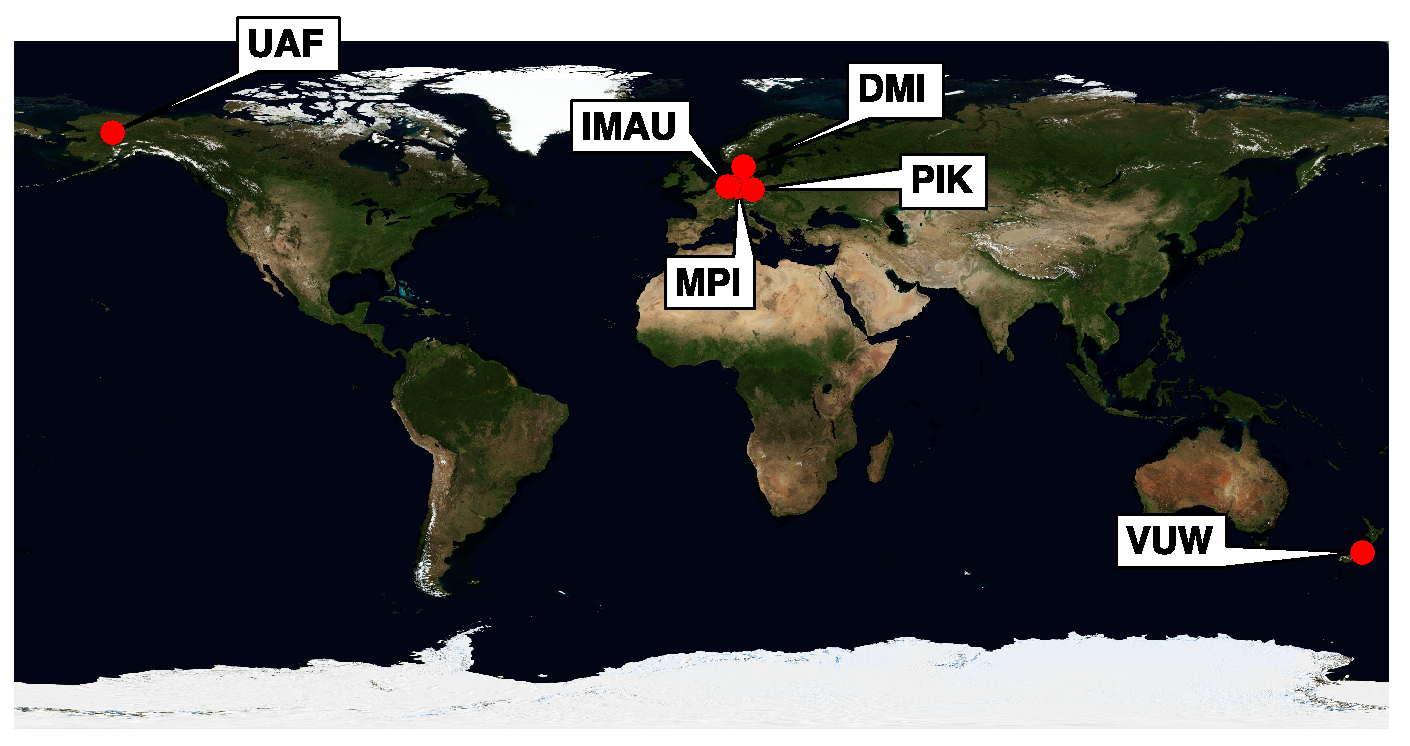
\includegraphics[width=0.75\linewidth]{pism-user-world}
     \end{center}
  \item developed here at UAF
  \item supported by NASA MAP and ARSC
  \item see \alert{www.pism-docs.org}
  \item \dots but just an example for this talk
  \end{itemize}
\end{frame}


\begin{frame}
  \frametitle{generating initial states using PISM}
  \begin{block}{some initialization schemes:}
    \begin{itemize}
    \item {\color{dark blue}{constant-climate}} steady-state using
present-day climate
    \item {\color{dark orange}{paleo-climate}} uses (imperfect) data from a full Ice Age cycle
    \item {\color{dark violet}{flux-corrected paleo-climate}} combines
paleo-climate with information about present-day ice thickness
    \end{itemize}
  \end{block}

  \begin{itemize}
  \item I'll mostly show Andy's Greenland runs on 2 km grid
  \end{itemize}
\end{frame}


\begin{frame}{validation metric: ice volume and ice thickness}

\begin{itemize}
\item the most common validation metric is ice volume
\item ice volume measurement based on ice thickness observation
\item PISM Greenland runs comparison:

\vspace{1em}

{\scriptsize{
\begin{tabular}{l c c c c}
\hline
  & observed & \color{dark blue}{constant-climate} & \color{dark orange}{paleo-climate}  & \color{dark violet}{flux-corrected}\\
\hline
\emph{ice volume}\\
initial volume\, [10$^{6}$\,km$^{3}$] & 2.93 & \color{dark blue}{3.18} & \color{dark orange}{3.37} & \color{dark violet}{X} \medskip \\

\emph{ice thickness}\\
avg abs.~difference [m] &  & \color{dark blue}{99} & \color{dark orange}{121} & \color{dark violet}{X}\\
rms difference [m] & & \color{dark blue}{199} & \color{dark orange}{244} & \color{dark violet}{X}\\
\hline
\end{tabular}
observed ice thickness is from Griggs \& Bamber (unpublished)
}}
\scriptsize
\item[\color{dark violet}{X}] = ice thickness used in ``flux-correcting'' is not available for validation
\normalsize
\bigskip

\item thus: volume is a weak metric because it averages out positive and negative thickness errors
\item how well do we know ice thickness?
\end{itemize}
\end{frame}


\begin{frame}{validation metric: gravimetric total mass changes}
  \begin{figure}
    \includegraphics<1>[width=0.9\textwidth]{ts_mass_2004-2010}
  \end{figure}
\end{frame}



\begin{frame}{validation: surface speeds}
  \vspace{-2em}

  \begin{figure}
    \includegraphics<1>[height=4.5cm]{csurf_insar_pism_all} \\
   \footnotesize{a) observed; b) constant-climate; c) paleo-climate; d) flux-corrected}
  \end{figure}
  
\begin{itemize}
\item values in m/a
\item observed = interferometric SAR $+$ feature-tracking \footnotesize (Joughin et al., 2010) \normalsize
\item some ``data assimilation techniques'' (inverse modelling of the observed velocities) give much better match to observed velocities \dots but it's not clear if time-evolution is better
\end{itemize}
\end{frame}



\begin{frame}{validation: surface elevation change 2003--2009}
 \begin{figure}
    \includegraphics<1>[height=4.25cm]{dh_2003-2009} \\
    \footnotesize{a) observed; b) constant-climate; c) paleo-climate; d) flux-corrected}
  \end{figure}

\begin{itemize}
\item values in m
\item observed = ICESat laser altimetry \footnotesize (S\o{}rensen, 2011) \normalsize
\end{itemize}
\end{frame}


\section{challenges}

\begin{frame}{we've come a long way baby?}
  \vspace{-.25cm}
  \begin{figure}
    1990s (20 km grid) \hspace{1.75cm} today (1 km grid)\\
    \includegraphics[height=7cm]{csurf-eismint-today}
  \end{figure}
\end{frame}


\section{questions?}


\end{document}
